\documentclass{standalone}
\usepackage{tikz}

\usetikzlibrary{patterns, positioning, arrows}


\begin{document}

    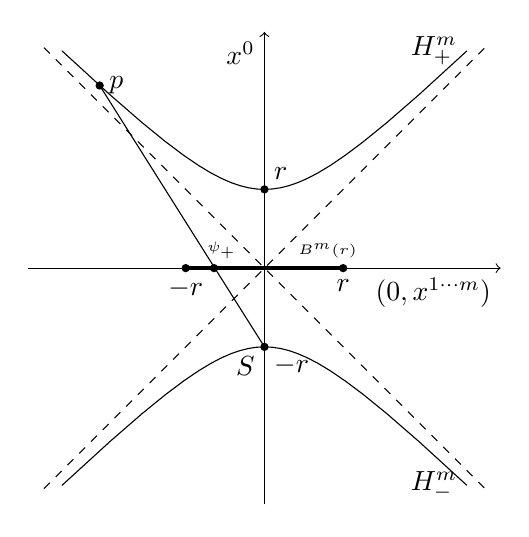
\begin{tikzpicture} %[>=Stealth] %修改箭头样式
%        \draw[lightgray, very thin] (-3,-1) grid (4,6); %作网格
        \draw[->] (-3,0) -- (3,0) node[below left] {$(0,x^{1\cdots m})$}; %作x轴并标上字母
        \draw[->] (0,-3) -- (0,3) node[below left]  {$x^{0}$}; %作y轴并标上字母
%        \node[below left] at (0,0) {$O$}; %标上原点字母
        \draw[domain = -1.2 : 1.2] plot ({tan (\x r)},+{sec(\x r)}) node[left] {$H^m_{+}$};
        \draw[domain = -1.2 : 1.2] plot ({tan (\x r)},-{sec(\x r)}) node[left] {$H^m_{-}$};
        \draw[line width = 1.5pt](-1,0)node[below]{$-r$} -- (1,0)node[below]{$r$};
        \fill (-1,0) circle (1.5pt); \fill (1,0) circle (1.5pt); \fill (-0.64,0) circle (1.5pt);
        \fill (0,1) circle (1.5pt) node[above right]{$r$};
        \draw[dashed] (-2.8,-2.8) -- (2.8,2.8);
        \draw[dashed] (-2.8,2.8) -- (2.8,-2.8);
        \fill (0,-1) circle (1.5pt) node[below left]{$S$} node[below right]{$-r$} coordinate (ss);
        \fill ({tan (-1.125 r)},{sec(-1.125 r)}) circle (1.5pt) node[right]{$p$} coordinate (pp);
        \draw (pp) -- (ss);
        \node[above right] at (-0.85,0) {\tiny $\psi_{+}$}; 
        \node[above] at (+0.8,0) {\tiny $B^m(r)$}; 
    \end{tikzpicture}

\end{document}